\section{Materials}
All the additive manufacturing technique described above can be applied, on theoretical grounds, to metallic materials in any form as well as to other classes of materials (see \cref{fig:materials-chart}). For the purposes of this report, we shall limit the discussion to two classes: pure metals and alloys powder. In the last part of this section, we describe in a more detailed way three specific metal alloys of particular interest to companies we collaborate with.
\begin{figure}[bt]
    \centering
    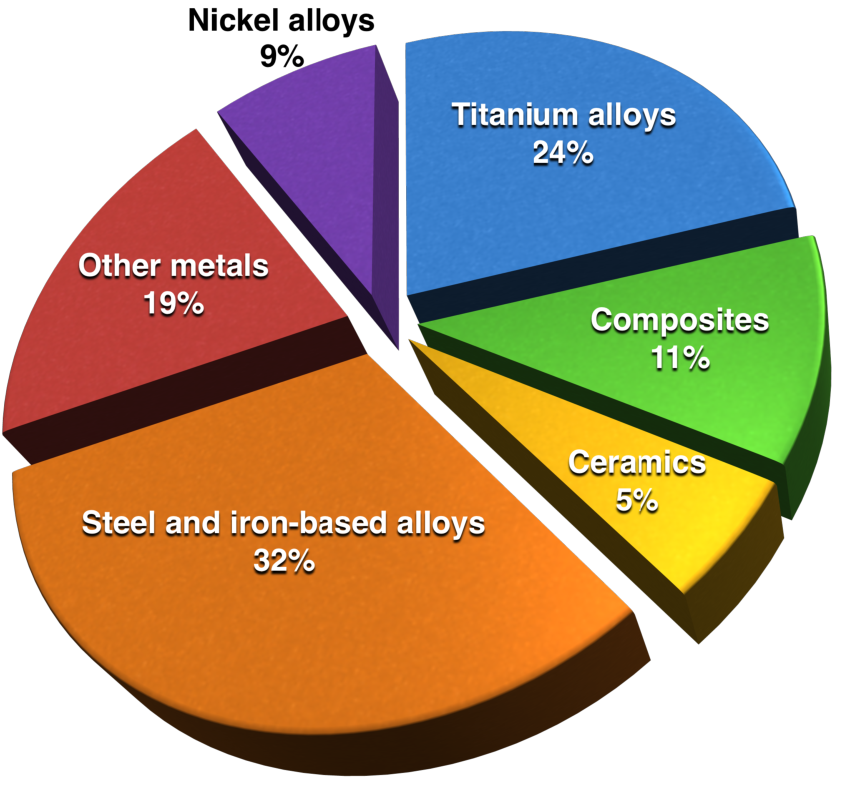
\includegraphics[width=0.5\textwidth]{materials-chart}
    \caption{Research interests on LM manufacturing of different materials, based on publications indexed by Web Of Science and ScienceDirect from 1999 to 2014. From \cite{Yap2015}.}
    \label{fig:materials-chart}
\end{figure}

\subsection{Common classes of materials}
\subsubsection{Pure metals}
Pure metals have been applied for various AM processes since the beginning. However, they are no more the focus of future development of AM technology mainly because of two reasons: firstly, pure metals are known to have relatively poor mechanical properties and, from a chemical point of view, they are more prone to corrosion and/or oxidation. Secondly, early attempts to processing pure metals with the laser sintering technique have been largely unsuccessful (i.e.\ poor overall quality of final products) and a real improvement has been possible only with first successful applications of LM. For example~\cite{Fischer2004}, LS processing of pure Ti samples showed that final products typically has an heterogeneous microstructure, which consists of cores of unmelted powder grains, melted surface of grains and residual voids; this means that the density of parts so obtained can be quite far from the level required to ensure good mechanical properties. For these reasons, currently industrial applications moved from LS to LM or LMD to build nonferrous pure metals components. It is worth noting, however, that recent studies~\cites{Krishna2007}{Xue2007} on a partial melting mechanism of pure metals such as Ti and Ta have demonstrated the interesting possibility of producing complex shaped porous structures with functionally graded porosity used for biomedical applications.

\subsubsection{Alloys powder}
The majority of the actual research (and subsequent applications) has been focused on powder alloys, based on metals such as Ti, Ni and Fe. Additive manufacturing of aluminum--based alloys might be the next research step, in order to face the difficulties related to the processing of nonferrous alloys with high reflectivity to laser energy. Almost all the work on AM of alloys powder is based on a complete melting mechanism, thus adopting the techniques of LS or LMD. Therefore, high laser source power is generally required to yield good bonding mechanism and obtain fully dense parts (excepts for porous materials if needed). Examples of lasers used for this purpose are \ce{CO2} powered lasers, Nd:YAG and fibre lasers. Besides the setup of the processing parameters, residual stresses and microstructures are two important aspects to take into account, as they are strongly influenced by large undercooling degree during rapid solidification, after the laser source has generated the molten pool. As proposed by Abe et al.~\cite{abe+01jmatproctech}, a possible way to solve these issues is the use of a dual laser scanning system; essentially, in this way one of the two laser can be used during a "preheating" phase before the actual melting or after the latter in a ``reheating'' phase.

%\subsubsection{Metal matrix composites}
%Metal matrix composites (MMC) can be classified as multicomponent systems, in which the metal acts as the binder while the ceramic material is the structural one. The idea of mixing metal and ceramic reinforcement is one of the most common practice in modern material science: putting together different materials to exploit the advantages of both and obtain a multicomponent system with new properties. MMC in fact exhibits an optimum combination between a simple metal matrix and stiffer and stronger ceramic material. Usually, MMC powders are obtained by mechanically alloying a mixture of different powder components (for example, with the technique called ``ball milling''\footnote{\textit{cit. 202 from Gu et al.}}). One of the most studied metal matrix composite for AM is \ce{WC}--\ce{Co} (tungsten carbide and cobalt)\footnote{\textit{cit. 203--207}}, since even with LS high density parts can be obtained, comparable with conventionally sintered hard metals.

%MMC just described are also called \emph{ex situ} MMC, because the ceramic reinforcing particles are added separately to the metal matrix. Recently, using the very AM technology, there has been the development of novel \emph{in situ} MMCs, in which the constitutions are synthesized directly during the process by chemical reactions. In this way, MMCs are thermodynamically stable systems and thus more suitable for high temperature applications. Moreover, interfaces between ceramic and metal have a smaller surface roughness, yielding to stronger interfacial bonding and in turn optimal mechanical properties of the final products\footnote{\textit{cit. 225}}.



%\subsection{Ni, Ti and Au based alloys}
\subsection{Nickel based superalloys}
A superalloy is a metallic alloy which can be used at high temperatures, often in excess of the absolute melting temperature. Resistance to creep and oxidation are the design criteria of prime interest. Superalloys can be based on iron, cobalt or nickel, with the latter being widely studied as best suited many industrial, high--performance applications such those required in the aerospace field.

The fundamental solutes in nickel based superalloys are aluminium and titanium, with a total concentration which is typically less than 10 atomic percent. This generates a two--phase equilibrium microstructure, consisting of gamma ($\gamma$) and gamma--prime ($\gamma'$) phases. It is the $\gamma'$ which is largely responsible for the elevated temperature strength of the material and its incredible resistance to creep deformation. The amount of $\gamma'$ depends on the chemical composition and temperature.%, as illustrated in the ternary phase diagrams below.

The $\gamma$ phase is a solid solution with a Face Centered Cubic lattice and a random distribution of the different species of atoms. By contrast, $\gamma'$ has a simple cubic lattice in which the nickel atoms are at the face-centres and the aluminium or titanium atoms at the cube corners, as the following picture shows schematically.
\begin{figure}[tb]
    \centering
    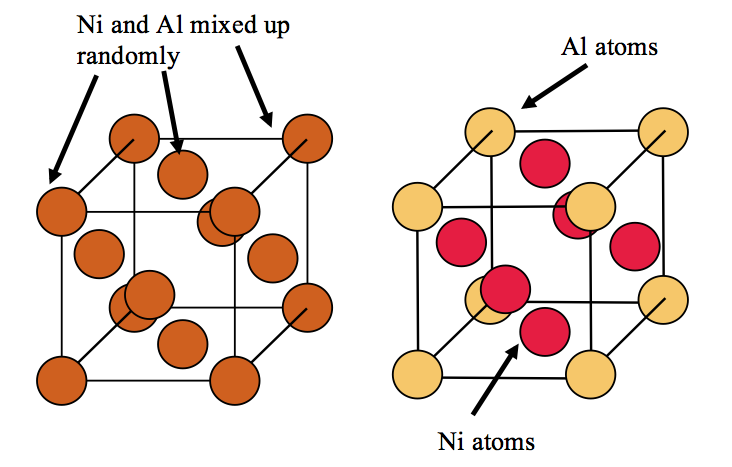
\includegraphics[width=0.65\textwidth]{Ni_structures}
    \caption{On the right, the structure of the $\gamma$ phase, a solid solution of Ni and Al atoms. The left scheme is the structure of the $\gamma'$. From: {\ttfamily\url{http://www.eng-atoms.msm.cam.ac.uk/}}}
    \label{fig:Ni_struct}
\end{figure}

This atomic arrangement has the chemical formula \ce{Ni3Al} or \ce{Ni3Ti}. However, as can be seen in the following phase diagram at \SI{1573}{K}, from the ($\gamma$+$\gamma'$)/$\gamma'$ phase boundary on the ternary sections of the Ni, Al, Ti  the phase is not strictly stoichiometric: there may exist an excess of vacancies on one of the sublattices which leads to deviations from stoichiometry or substitutional defects may be present, i.e.\ some of the Ni atom may occupy Al sites or vice--versa. 

\begin{figure}[t]
    \centering
    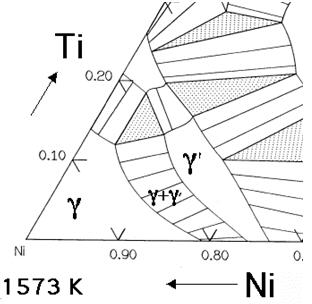
\includegraphics[width=0.4\textwidth]{TernaryPhase}
    \caption{Ni-Al-Ti ternary phase diagram at \SI{1573}{K} with the $\gamma$, $\gamma'$ and coexistence regions indicated. From From: {\ttfamily\url{http://www.eng-atoms.msm.cam.ac.uk/}}}
    \label{fig:Ni_phase}
\end{figure}

One of the most important properties of these alloys is their strength up to very high temperatures. More precisely, these alloys show high yield strengths (usually denoted by $\sigma_y$) and at first these values are independent on temperature. An explanation of this peculiar property lies in the structure of the two phases: both have a cubic lattice with similar lattice parameters and the $\gamma$ phase forms the matrix in which the $\gamma'$ precipitates. In this ``transition'' cubic symmetry is preserved and thus cell edges of the $\gamma'$ are exactly parallel to the corresponding edges of the $\gamma$ phase. Furthermore, because their lattice parameters are similar, when the precipitate size is small, there is a little lattice misfit between the two phases . Dislocations in the $\gamma$ nevertheless find it difficult to penetrate $\gamma'$, partly because the latter is an atomically ordered phase. The order interferes with dislocation motion and hence strengthens the alloy.

Also the mismatch between the lattice parameters of the two phase plays quite an important role: it promotes the stability of the microstructure at high temperature. This is mainly due to the fact that the $\gamma$ and the $\gamma'$ belong to almost equal crystal structure and thus the $\gamma/\gamma'$ interface energy is quite low. The mechanism of precipitate coarsening (i.e.\ the Oswald ripening) is thermodynamically driven by the minimisation of the interface energy and therefore the more coherent is the interface (i.e.\ the smaller its surface free energy), the more stable is the microstructure, because especially at high temperature it does not happen that a precipitate of a solid phase grows at the expense of another one.

Commercial superalloys contain more than just Ni, Al or Ti. Essential resistance to oxidation is promoted also by the presence of chromium besides aluminum and small quantities of yttrium help the oxide layer to be commensurate with the substrate. Furthermore, when dealing with polycrystalline superalloys the addition of boron and zirconium results in reducing the grain boundary energy, which in turn improve overall creep strength. There are, naturally, limits to the concentrations of these element that can be added without inducing precipitation or promoting the formation of brittle phases.


\subsection{Titanium alloys}
Titanium alloys are among the most important of the advanced materials that are essential in several fields of applications, from aerospace to biomedical. This is because of an excellent combination between mechanical properties and, for example, a formidable resistance to corrosion exhibited by titanium alloys. On the other hand, the high cost of production of these alloys compared to competing materials is one of the main reasons negating their widespread use.

Like a number of other metals titanium can crystallize in various crystal structures. The complete transformation from one into another crystal structure is called ``allotropic transformation''.

Pure titanium, as well as the majority of titanium alloys, crystallizes at low temperatures in a modified ideally hexagonal close packed structure, called $\alpha$ titanium. At high temperatures, however, the body-centered cubic structure is stable and is referred to as $\beta$ titanium. The $\alpha-\beta$ transition temperature for pure titanium is \SI{882}{\celsius}. The atomic unit cells of the hexagonal close packed (hcp) $\alpha$ titanium and the body-centered cubic (bcc) $\beta$ titanium are schematically shown in Fig.~\ref{fig:Ti_structures} with their most densely packed planes and directions highlighted.
The existence of the two different crystal structures and the corresponding allotropic transformation temperature is of central importance since they are the basis for the large variety of properties achieved by titanium alloys.
\begin{figure}[b]
    \centering
    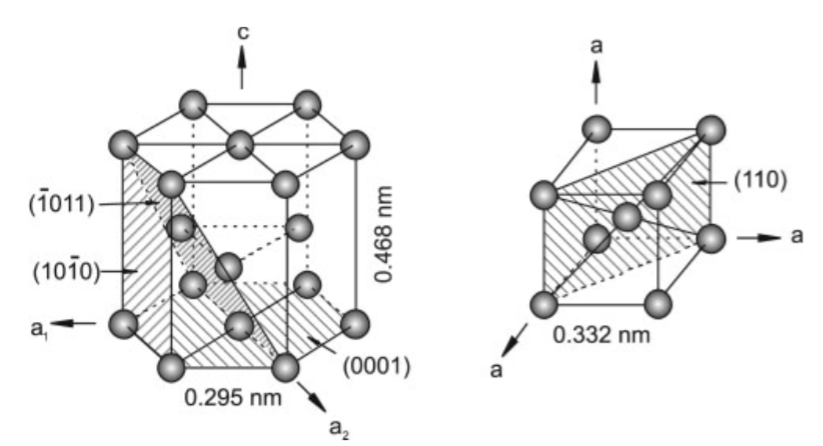
\includegraphics[width=.6\textwidth]{Ti_structures}
    \caption{Crystal structure of HCP $\alpha$ and BCC $\beta$ phase~\cite{LeyensBOOK2003}.}
    \label{fig:Ti_structures}
\end{figure}

Depending on their influence on the $\beta$ transition temperature, the alloying elements of titanium are classified as neutral, $\alpha$--stabilizers, or $\beta$-stabilizers (Fig.~\ref{fig:Ti_alloys}). The $\alpha$--stabilizing elements extend the $\alpha$ phase field to higher temperatures, while $\beta$--stabilizing elements shift the $\beta$ phase field to lower temperatures. Neutral elements have only minor influence on the transition temperature. Apart from the regular alloying elements, there are also primarily nonmetallic elements on the order of few \SI{100}{ppm} present as impurities.
\begin{figure}[tb]
    \centering
    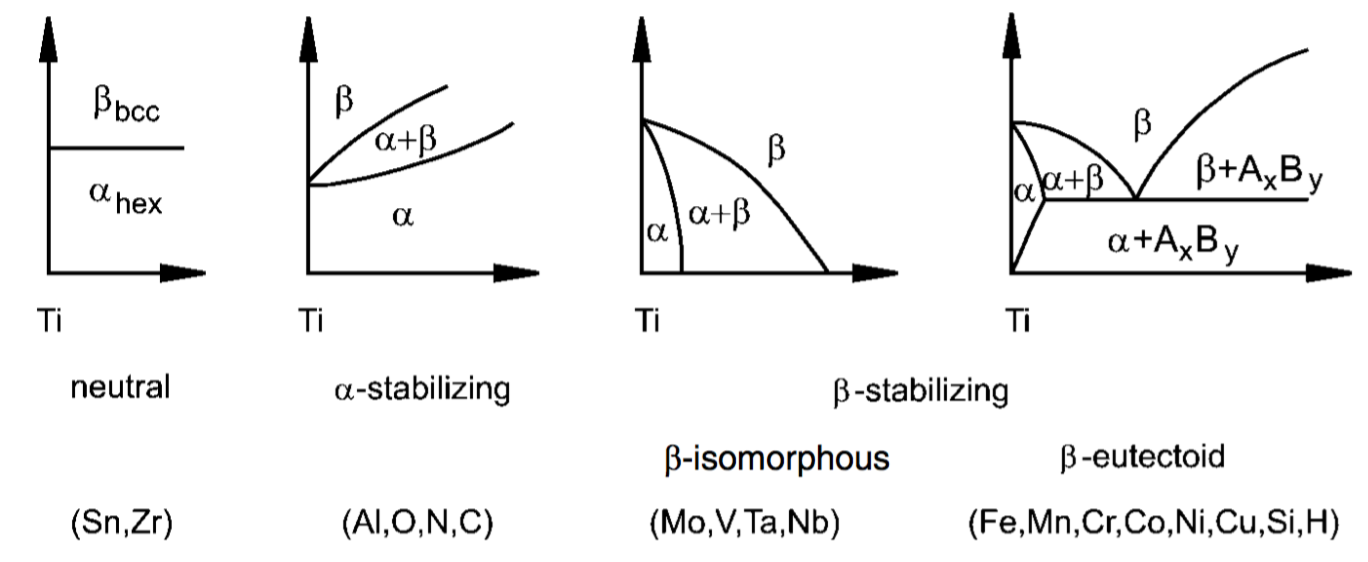
\includegraphics[width=.65\textwidth]{Ti_alloys}
    \caption{Schematic picture of the influence of alloying elemnents on Ti phase diagrams~\cite{LeyensBOOK2003}.}
    \label{fig:Ti_alloys}
\end{figure}

Among the $\alpha$--stabilizers, aluminum is by far the most important alloying element of titanium. The interstitial elements oxygen, nitrogen, and carbon also belong to this category. In addition to extending the a phase field to higher temperatures, the $\alpha$--stabilizers develop a two--phase $\alpha+\beta$ field. $\beta$--stabilizing elements are subdivided into $\beta$--isomorphous and $\beta$--eutectic elements. Of these, the $\beta$--isomorphous elements such as Mo, V, and Ta are by far more important due to their much higher solubility in titanium. In Fig.~\ref{fig:Ti_phase} a schematic three--dimensional diagram shows the most stable phases with respect to the added concentration of stabilizers (here only Al and V are shown).
\begin{figure}[bt]
    \centering
    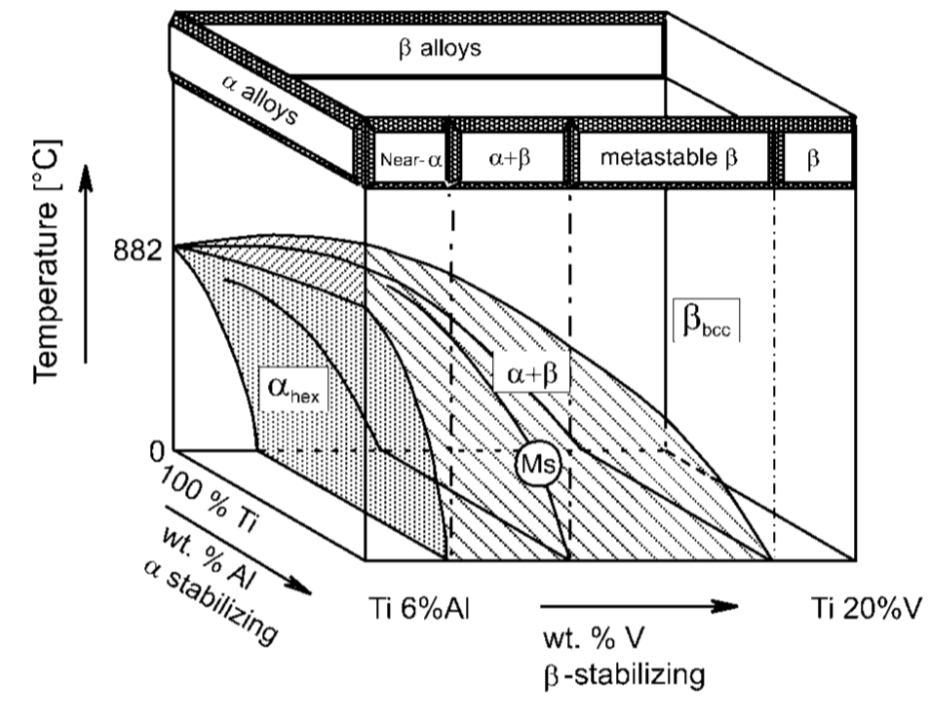
\includegraphics[width=.65\textwidth]{Ti_3Dphase}
    \caption{Three-dimensional phase diagram to classify Ti alloys~\cite{LeyensBOOK2003}.}
    \label{fig:Ti_phase}
\end{figure}

The microstructure of conventional titanium alloys is primarily described by the size and arrangement of the two phases $\alpha$ and $\beta$. The two extreme cases of phase arrangements are the lamellar microstructure, which is generated upon cooling from the $\beta$ phase field, and the equiaxed microstructure, which is a result of a recrystallization process. Both types of microstructure can have a fine as well as a coarse arrangement of their two phases. Generally, the different microstructures are generated by thermomechanical treatments, considered as a complex sequence of solution heat treatment, deformation, recrystallization, aging, and annealing for stress relief.

An important point for thermomechanical treatment is the $\beta$--transition temperature ($T_\beta$), since it separates the single $\beta$ phase field from the two--phase $\alpha+\beta$ field. Lamellar microstructures are a result of simple cooling from temperatures above $T_\beta$. Once the temperature falls below the $T_\beta$, $\alpha$ phase nucleates at grain boundaries and then grows as lamellae into $\beta$ grains.
Depending on the cooling rate, the lamellae are either fine or coarse: slow cooling from the $\beta$ phase field results in pure lamellar microstructures, with the lamellae becoming coarser with reduced cooling rate. Rapid quenching, instead, leads to a martensitic transformation of the $\beta$ phase, resulting in a very fine needle--like microstructure.

To generally improve the properties of materials, and titanium alloys in particular, there are essentially two ways to proceed: alloying and processing. Recently a third option has gained importance: the production of composite materials. %(also called Metal Matrix Composites, already discussed in the previous section).

Alloying lays the basis for an increase in strength (e.g.\ solid-solution strengthening, age hardening), allows the generation of ordered structures (e.g.\ intermetallic compounds of titanium and aluminum), determines most of the physical properties (e.g.\ density, elastic modulus, coefficient of thermal expansion), and largely controls the chemical resistance of the material (corrosion, oxidation).

Processing allows the careful balancing of the property profile of materials. Depending on the specific property profile required for the final application, different microstructures can be generated for titanium alloys by means of thermomechanical treatment to optimize for strength (solid solution strengthening, dispersion strengthening, grain boundary strengthening, texture hardening), ductility, toughness, superplasticity, stress corrosion, creep resistance, etc. The processing techniques of rapid solidification and mechanical alloying extend the spectrum of potential alloy compositions.






%%% Section on Au alloys (rewritten)
% !TEX root = ../Main.tex
%!!!!!!!!!!!!!!!!!!!!!%
%%%%% OLD VERSION %%%%%
%!!!!!!!!!!!!!!!!!!!!!%
%
%%%\subsubsection{Gold and its ``colours''}
%%%From ancient times, gold has been used mostly in decorative items, and the colour of gold plays an important role in this application field. Gold and copper are the only two metals that exhibit colour and, thanks to this property, gold alloys can be made to assume a range of colours by varying the alloying additions. Human history is rich in examples of the usage of gold and its colours for different purposes: silver--gold (roughly 70\% of gold and 30\% of silver) was employed by Lydians to make coins and red gold was used by goldsmiths in pre--Columbian cultures\footnote{Ref.~3 Cretu1999}. Today, various ``colours'' of gold are available with the main objective of making jewellery.
%%%
%%%The formation of colour in metallic elements and their alloys can be explained by means of the band theory. When metal and light interact, electrons from the metal surface situated either below or on the Fermi level absorb photons and are promoted to excited states. The efficiency of the absorption and re--emission of light depends on the atomic orbitals from which the energy band originated. In the case of gold and copper, the efficiency decreases with increasing energy, resulting in yellow reflectivity (i.e.\ a larger contribution to reflection arises from the low--energy wavelengths of the light spectrum). In silver, in spite of a very similar electronic structure, transition of electrons above the Fermi level requires energy in excess of that of the violet end of the visible spectrum: all the visible spectrum is evenly reflected, resulting in the characteristic gray metallic color\footnote{Ref.~Cretu1999}.
%%%
%%%Alloying additions to gold and copper can create various colours. It is less well known, however, that gold alloys can have colours which are surprisingly different to the conventional alloys, as in the case of blue, black or purple gold alloys.
%%%Gold coloured alloys can be classified in three main categories:
%%%\begin{enumerate}
%%%    \item Au--Ag--Cu system;
%%%    \item Intermetallic compounds;
%%%    \item Surface oxide layers\footnote{This category will not be discussed here, but details can be found in referenced literatures. For example, see Refs.~47, 48, 49 and 50 of Cretu1999.}.
%%%\end{enumerate}
%%%
%%%%We will discuss in more detail the first and describe briefly intermetallic compounds, while leaving the third class to the referenced literature\footnote{See, for example, Refs.~47, 48, 49 and 50 of Cretu1999.}.
%%%
%%%\paragraph{Au--Ag--Cu system}
%%%This system is the basis of the most used gold alloys with applications in jewellery and, though less and less common, dental prosthesis. Colours of yellow, green and red can be obtained with different ratios of Au:Ag:Cu (see Fig.~\ref{fig:AuAgCu}).
%%%\begin{figure}[tb]
%%%    \centering
%%%    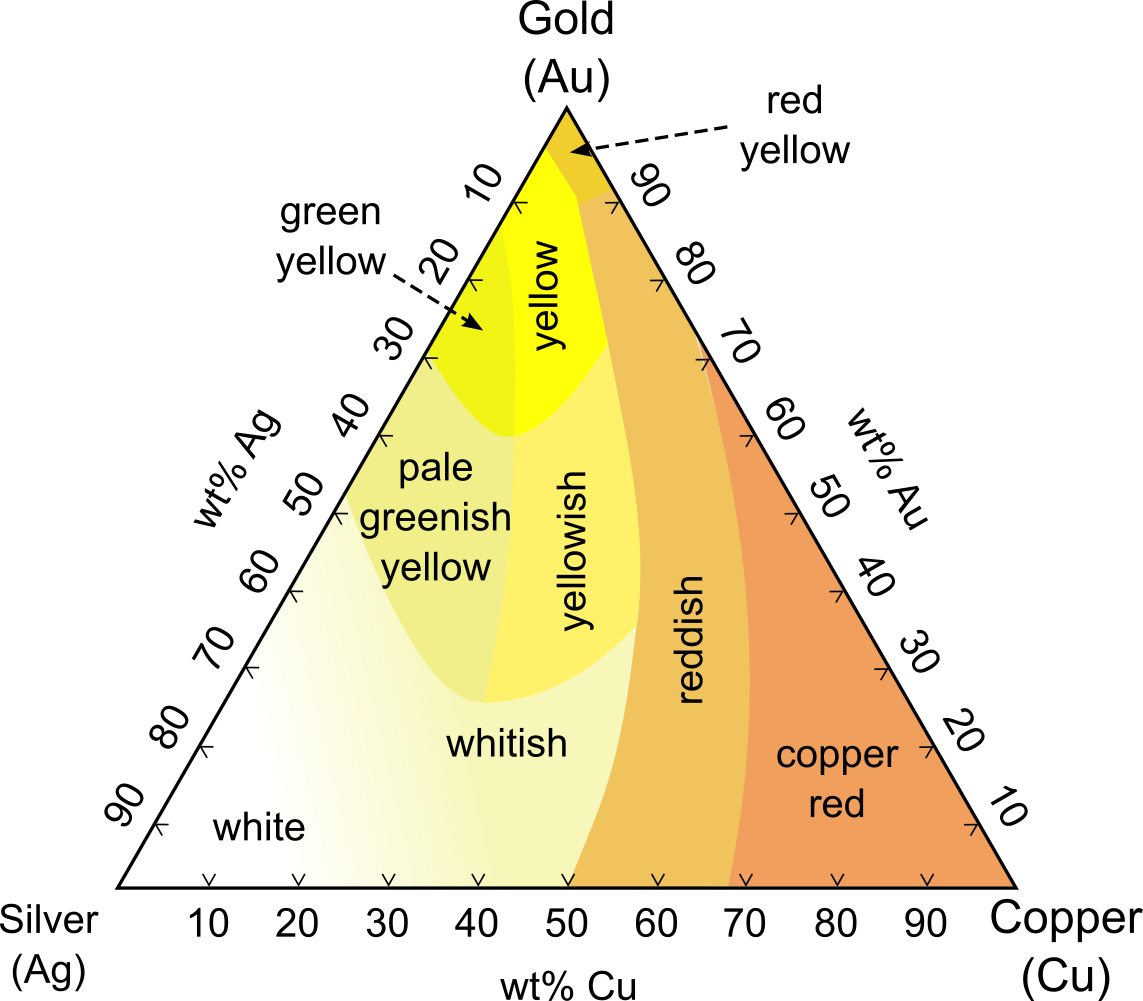
\includegraphics[width=.65\textwidth]{Ag-Au-Cu-colours}
%%%    \caption{Approximate colours of Au--Ag--Cu alloys, which are commonly used in jewelry making. From \href{https://commons.wikimedia.org/wiki/File:Ag-Au-Cu-colours.png}{\ttfamily Wikimedia}.}
%%%    \label{fig:AuAgCu}
%%%\end{figure}
%%%White gold is also based on this system, by adding alloying elements known for their bleaching characteristics such as nickel, palladium or manganese.
%%%
%%%Generally, additions of copper give a reddish tint to the alloy, and additions of silver make the alloy greenish, in accordance with band theory\footnote{The addition of silver to the Au--Cu alloy causes a widening of the energy gap that the electrons have to overcome to reach an energy state above the Fermi level. The wider the gap, the higher the energy absorbed from the incident light, and therefore the reflectivity increases also for the green region of the spectrum.}. An extensive study of the ternary alloy Au--Ag--Cu and its metallurgy, including order--disorder phenomena, can be found in REFS\footnote{Refs.~13,14,15,16 of Cretu1999.}.
%%%
%%%\paragraph{Intermetallic compounds}
%%%The term ``intermetallic compounds'' indicates a particular group of materials whose properties are much different from the individual metallic components. These compounds can be defined as an intermediate phase in an alloy system, with a narrow range of homogeneity and rather simple stoichiometry.
%%%
%%%In this category fall some of the less known coloured golds, such as purple gold and blue gold. Among these, the best known is \ce{AuAl2}, which is formed by about 80\% of gold and 20\% of aluminum\footnote{Ref.~34 Cretu1999} and exhibits a light purple colour, while \ce{AuIn2} and \ce{AuGa2} are used for their clear blue hues.
%%%
%%%The intermetallic compounds behave in some ways
%%%like pure metals, which makes it possible to calculate their band structures, but they are usually brittle materials and their use in traditional jewellery virtually impossible, though they can be faceted and used as gemstones or inlays.
%%%
%%%
%%%
%%%%\paragraph{Surface oxides}


\subsection{Gold alloys}
Gold is an element with one of the most unique spectrum of properties and for this reason its use is particularly widespread, not only for luxury goods like jewelry, but also in many other technical applications despite its high price.
From the chemical point of view it is the most “noble” of all metals: it does not corrode or oxidize and its stability towards influences from a variety of external conditions (be it natural, biomedical or technical) persists up to high temperatures. Moreover, it possesses high electrical and thermal conductivity and, from a mechanical point of view, is very soft, highly malleable and ductile at room temperature. Also optical properties play a crucial role for its applications: in its pure form gold shows a rich yellow color, but gold alloys can be made to assume a range of colours by varying the alloying additions. Human history is rich in examples of the usage of gold and its colours for different purposes.

In almost all areas of application, however, gold cannot be used in its pure form. It needs to be alloyed with other elements, usually metals, to adjust specific properties. For most applications, pure gold is simply too soft. For several applications, the properties of the pure gold need to be maintained as much as possible, for example, bonding wires in electronics or high carat gold jewelry\footnote{Caratage is defined as the fraction of pure gold present in a certain alloy. That is: 24 carat gold (24kt) = 100 wt\% Au, while $X$kt = $(X\times 100)/24$ wt\% Au.}.

The starting point for any kind of metallurgical processing not only for gold is provided by phase diagrams. The most common and used binary and ternary alloys of gold have been extensively studied and reviewed~\cite{OkamotoBOOK1987,PrinceBOOK1990,TernaryAlloyBOOK2006}. In this section we try to give a summary of the metallurgical approaches of gold alloying adopted in many fields of applications, with particular focus to grain refinement and solution strengthening.


\subsubsection{Grain refinement}
Grain refinement or grain--size control is the fundamental process applied routinely to all industrial applications of gold alloys. The list of advantages of a fine--grained material over a coarse--grained one is long and well documented:
\begin{itemize}
    \item increase of strength, malleability and ductility, as well as work--hardening effectiveness during cold--working process;
    \item increase of chemical homogeneity due to less pronounced alloying elements segregation. This in turn has a positive impact on corrosion resistance and susceptibility to embrittlement and crack formation in casting processes;
    \item an improvement of surface characteristics and finishing properties, mainly of interest for decorative and jewelry applications.
\end{itemize}

The only disadvantage provided by fine--grained material occurs at high temperatures where a loss of strength and reduction of creep resistance, due to a change of prevailing deformation mechanisms.

Grain--size control during material processing involves two particularly important steps: \textbf{solidification} after melting and \textbf{annealing} after cold--working.

Grain refinement during solidification mainly is concerned with promoting the formation of a larger number of nuclei for crystal growth from the molten state. This can be achieved by additions of particular elements with higher melting points with respect to the metal and low solubility in solid gold, such as iridium, ruthenium and rhenium, to cite a few~\cite{Nielsen1966}.
The required amount of the additions depends on alloy composition and can vary between \num{50} and \SI{1000}{ppm}. Higher amounts are not meaningful, since no further grain refining effect is usually observed.

Grain refining additions usually are introduced via carefully prepared base metal master alloys, for example Cu--10\% Ir, which need to offer a good liquid and solid solubility for the grain refiner, to provide a homogeneous distribution in the master alloy.

Apart from alloy additions, grain size during solidification is also influenced by processing~\cite{Ott1981}. Cold pouring of molten metal is frequently applied, keeping both metal and mould at low temperatures. This enhances crystal nucleation and retards crystal growth, leading to more fine--grained castings. Mould agitation or vibration support the homogeneous distribution of nuclei and ``mechanically'' refine the structure by breaking up the branches (dendrites) of growing crystals. 


During cold--working processes, the microstructure of a metal becomes strongly distorted: the material is strengthened and ductility is reduced to very low levels after heavy deformation. Complete or partial annealing then is carried out to recover ductility. For sufficiently high annealing temperature and time, the material recrystallizes, which involves nucleation and growth of new grains of regular shape.

Grain refinement during the annealing stage after deformation is mainly based on two mechanisms: increase of the number of recrystallization nuclei in the deformed microstructure and, more importantly, the decrease of grain growth velocity. For gold alloys, some of the additions that have been mentioned above as grain refiners during solidification can also promote the formation of recrystallization nuclei. However, if the growth of the nuclei is not inhibited as well, the described mechanism alone does not necessarily lead to a fine--grained microstructure. In extreme cases it may even have an adverse effect on grain size, namely if excessive growth of a few number of preferentially formed nuclei occurs. Furthermore, a fine--grained recrystallized structure energetically is not stable and tends to coarsen during prolonged annealing.

For all these reasons, the decrease of grain growth velocity by specific alloying additions is always of high importance. Impurities as well as alloying additions with low solubility in the metal matrix can reduce the grain boundary mobility drastically~\cite{Humphreys2004,Lucke1957}, because they tend to segregate to grain boundaries and therefore need to be able to move together with them during recrystallization and grain growth. This requires time and temperature--dependent diffusion processes to occur, which slows down recrystallization and grain growth kinetics.




\subsubsection{Strengthening mechanisms}
Deformation of any metal takes place by the sliding of crystal planes over each other through the movement of dislocations. Any distortion of the crystal lattice or any obstacle in the lattice increases the force required to move the dislocations through the lattice. Hence this leads to an increase of hardness or strength but usually also to a decrease of deformability. \Cref{fig:Au-hardness} gives an overview of the hardness increase in binary gold alloys depending on the type and amount of alloying element added.
\begin{figure}[bt]
\begin{center}
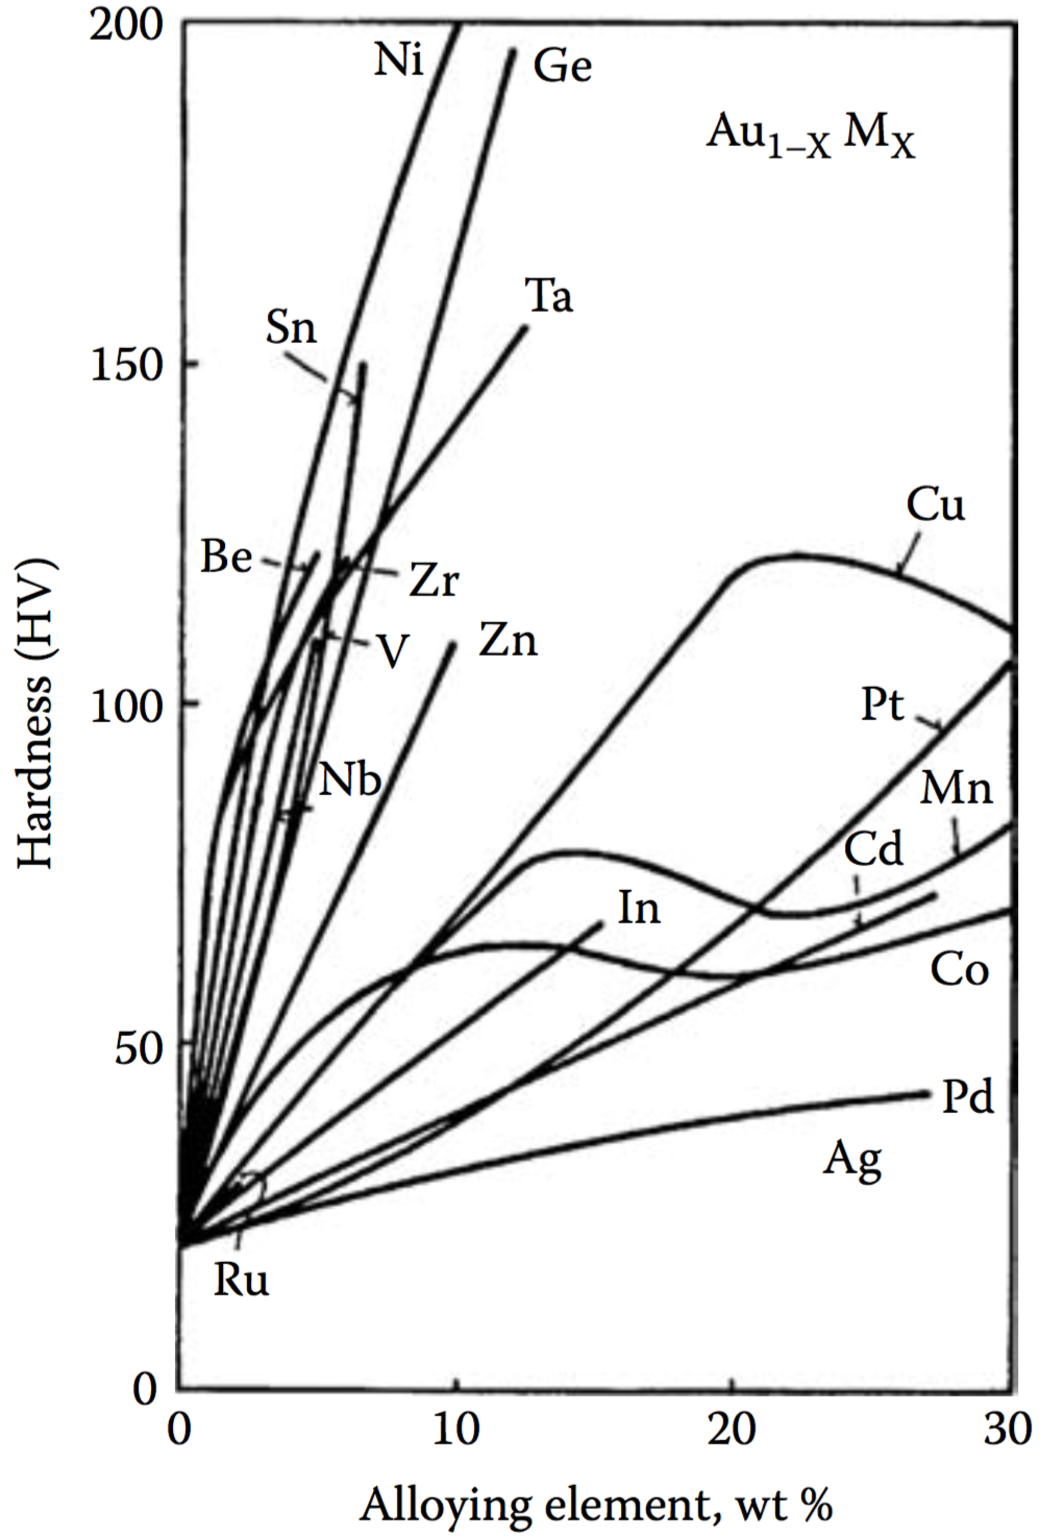
\includegraphics[height=.45\textheight]{Au-hardness}
\caption{Hardness trends in binary gold alloys depending on the type and amount of addition in weight \%~\cite{MetalPocketbook1995}. Units on hardness are expressed according to the ``Vickers hardness test'', that is: $HV=\text{force}/\text{area} = [\si{kgf}]/[\si{\square\milli\metre}]$.}
\label{fig:Au-hardness}
\end{center}
\end{figure}

The largely different dependencies are related to the different prevailing strengthening mechanisms, as well as the particular microstructural condition the material is in. Among these mechanisms, we mention: \textit{solid solution hardening}, \textit{order--disorder transformation hardening} and \textit{precipitation hardening}.

The last two mechanisms are reversible processes, since the material can be brought back to the ``nonhardened'' state by a homogenization heat treatment. These mechanisms are also usually referred to as \textit{age hardening}.

For the sake of completeness, we also cite the irreversible mechanism of \textit{dispersion hardening}, which is based on the irreversible formation of finely dispersed particles, mainly oxides (but also carbides or borides), by reaction of alloying elements with oxygen (or carbon/boron). This often involves special processing routes like internal oxidation or powder metallurgy.

\paragraph{Solid solution hardening.} This mechanism involves dissolution of alloying elements in solid gold, which can either replace gold atoms in the crystal lattice (as substitutional defects) or can fill in the small gaps between gold atoms in the crystal lattice (interstitial solid solution hardening).

The effect of solid solution hardening increases with the extent of lattice distortion associated with an alloying addition; thus the larger is the difference in atomic size between the host metal and the added element, the more prominent is this effect. This partially explains qualitatively the dependence of hardness on the Ag-Cu ratio in the Au-Ag-Cu ternary system, which forms the basis for many common jewelry (mainly for gold ``color spectrum'', \cref{fig:AuAgCu}) and dental alloys.
\begin{figure}[tb]
    \centering
    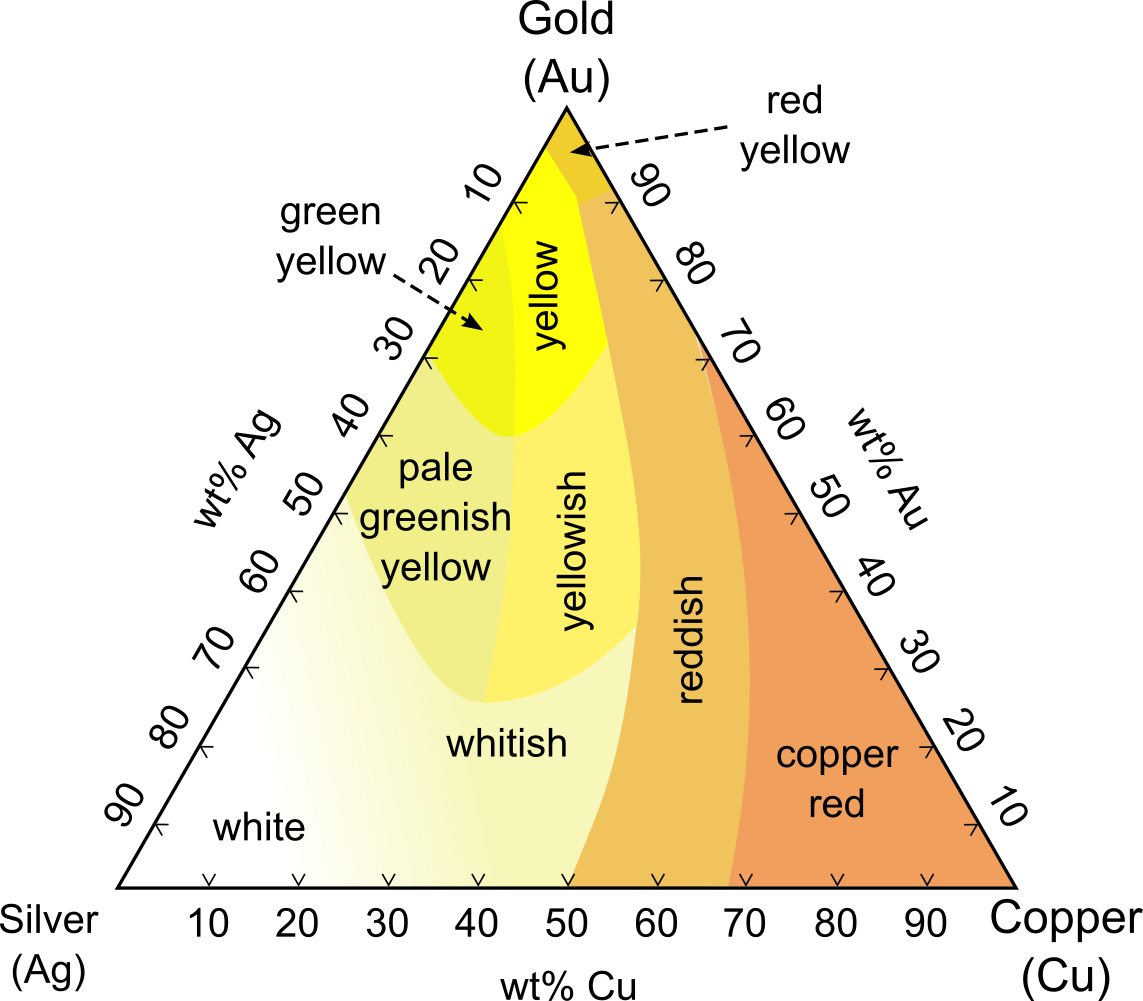
\includegraphics[width=.6\textwidth]{Ag-Au-Cu-colours}
    \caption{Approximate colours of Au--Ag--Cu alloys, which are commonly used in jewelry making. From \href{https://commons.wikimedia.org/wiki/File:Ag-Au-Cu-colours.png}{\ttfamily Wikimedia}.}
    \label{fig:AuAgCu}
\end{figure}

Gold is only slightly larger than silver, while copper atoms are $\sim 12\%$ smaller than gold: this explains why Cu is more effective in in strengthening of gold by subsitutional solid solution. On the other hand, Ag is completely soluble in Au at all temperatures and for any composition, while Cu is only miscible down to $\sim\SI{410}{\celsius}$: below this point, some intermetallic phases form, which give rise to additional hardening effects by precipitation hardening. Besides Ag and Cu, also palladium and platinum (soluble at any composition only at high temperatures) are largely used to induce solid solution strengthening. However, similarly to Ag, the strengthening effect of Pd and Pt is only small or moderate and usually further treatments are necessary to obtain the alloy with desired properties.
    




\paragraph{Order--disorder transformation hardening.} Due to the lowering of temperature during alloy processing, the atoms can arrange themselves in an ordered solid solution (also referred to as intermetallic compounds or intermediate phases), where different atoms occupy strictly defined lattice sites. Here strengthening is caused by the related elastic distortions, but also because the movement of dislocations is considerably more difficult because the ordered state needs to be preserved.

In the Au-Cu system, the intermediate phases responsible of this mechanism are \ce{CuAu}, \ce{CuAu3} and \ce{Cu3Au}.
The most important one is the phase occurring below \SI{410}{\celsius} at the composition for which the ratio Au:Cu is 1: alternating layers of Au and Cu form a face--centered tetragonal phase (\ce{AgCu} I) stable below \SI{385}{\celsius}, while an orthorombic phase is stable between \SI{385}{\celsius} and \SI{410}{\celsius} (\ce{AgCu} II). When Au:Cu ratio approaches 1:3, two versions of \ce{AuCu3} form with another ordered face--centered cubic symmetry (Cu atoms on lattice faces and Au atoms on lattice edges).

This hardening mechanism is a very important feature for many carat gold jewelry~\cite{Chaston1971:31GoldBook} and dental alloys~\cite{Laberge1979:35GoldBook}. It can be obtained either by slow cooling from high temperatures or by an aging period in the temperature range between \numlist{150;400} \si{\celsius}.
\begin{figure}[t]
    \centering
    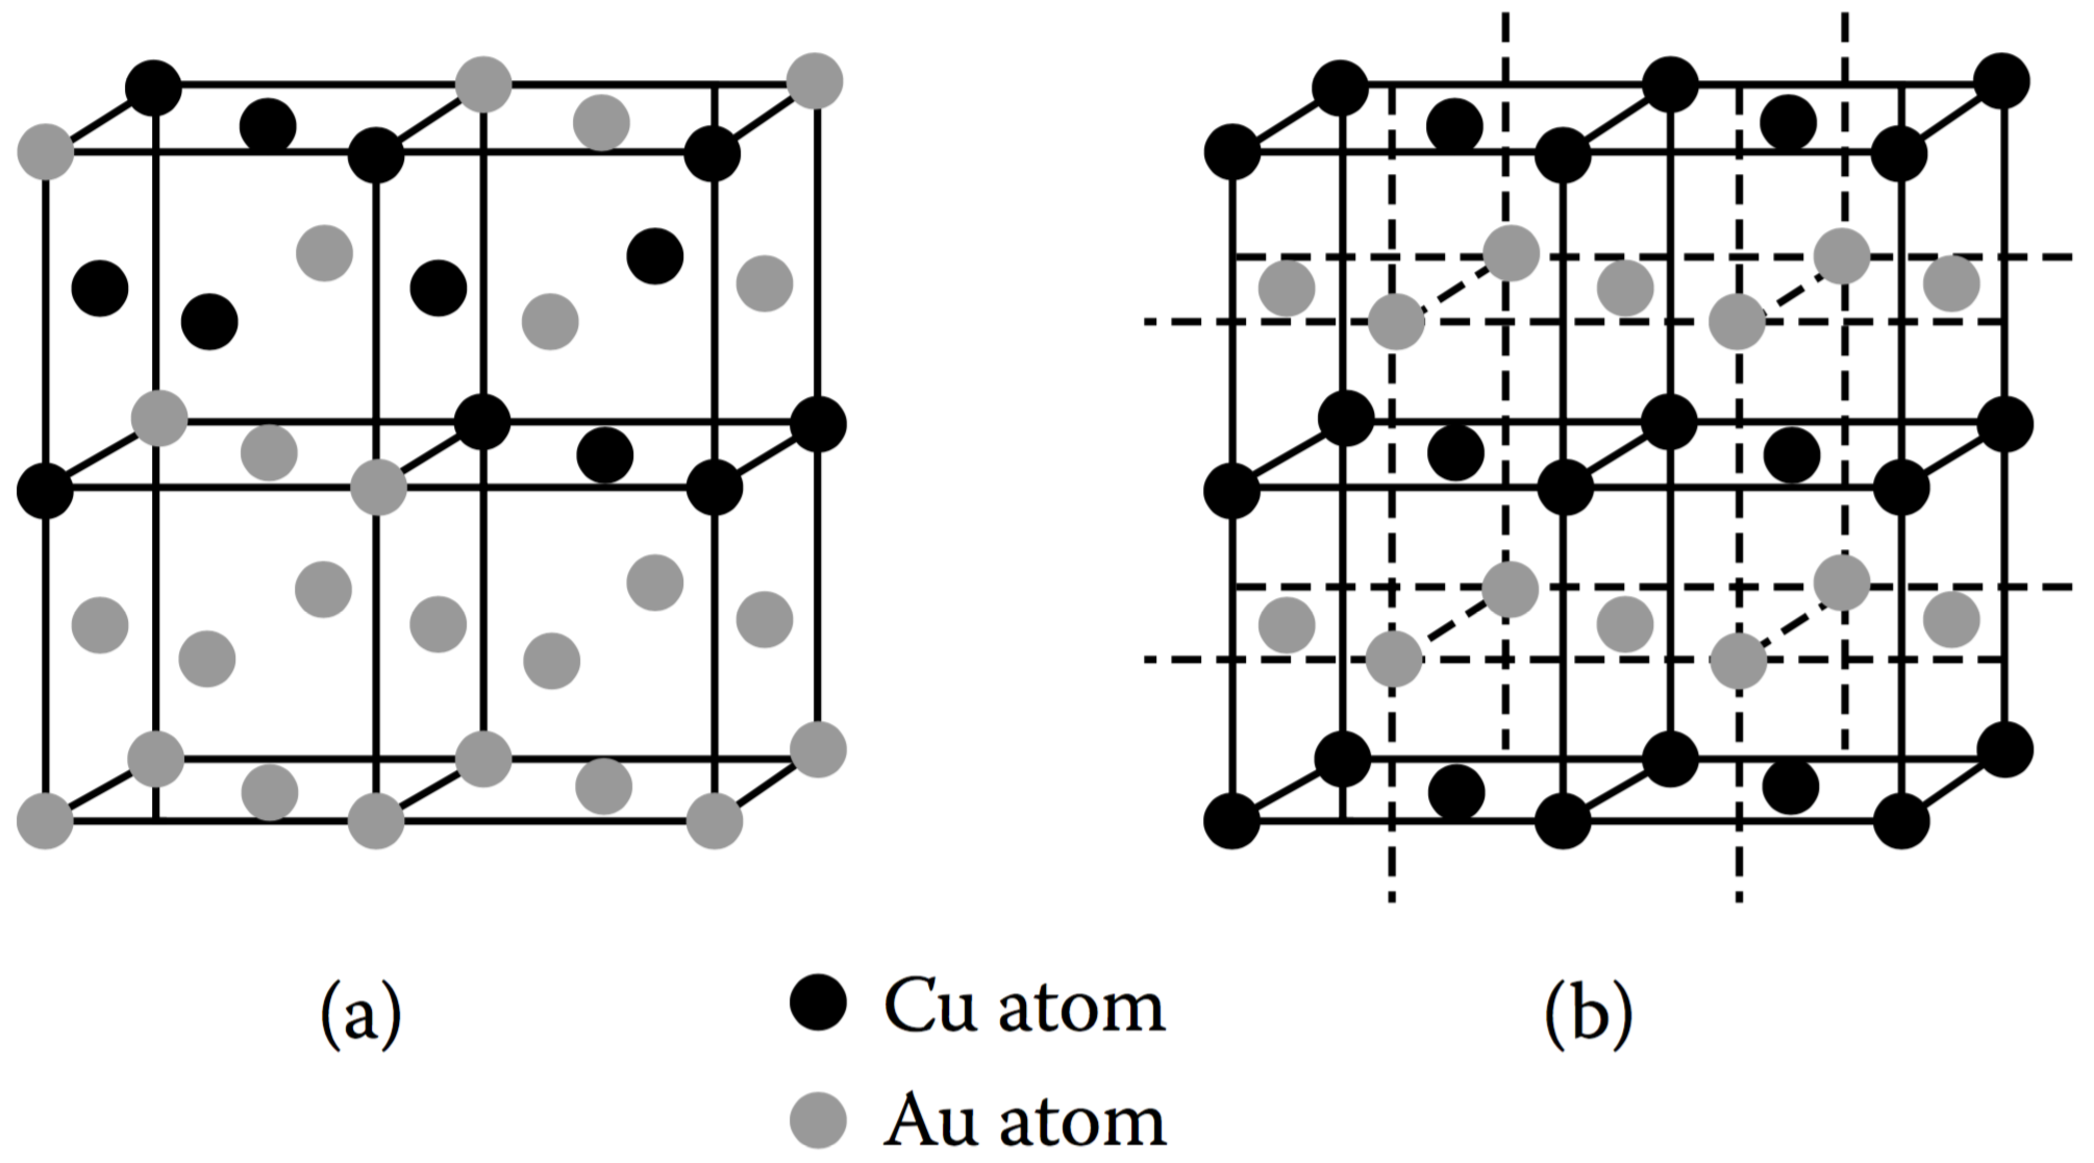
\includegraphics[width=.7\textwidth]{Au-order-disorder}
    \caption{(a) Crystal structure of the disordered solid solution in FCC \ce{AuCu}. (b) Crystal structure of the ordered face--centered tetragonal phase, \ce{AgCu}~\cite{Suss2004}.}
    \label{fig:order-disorder}
\end{figure}






\paragraph{Precipitation hardening.} 
The prerequisite for the activation of this mechanism is the reduced solid solubility of an alloying element in the metal matrix. Solid solubility generally decreases with temperature, thus this class of alloying elements can be precipitated by particular heat treatment as finely dispersed particles.

For binary gold alloys, this is the case of Au with Co, Cr, Fe, Mn and many others~\cite{OkamotoBOOK1987}. It can occur for several reasons:
\begin{itemize}
    \item the system behaves as a series of solid solutions at high temperatures, but as temperature decreases a miscibility gap opens up for certain compositions. This is the case of the Au-Ni, Au-Pt systems;
    \item systems in which a limited mutual solubility is present over the whole temperature range, like Au-Co and Au-Cr;
    \item alloy systems that present similar features as above, but where more than one intermetallic phase can occur.
\end{itemize}

Of course, also in more complex systems, like ternary or quaternary alloys, this hardening mechanism can occur. In all the cases, the system is subject to both an heat treatment and an aging period, which should comprise the following steps:
\begin{enumerate}
    \item an homogenization phase useful to dissolve all the alloying elements in the gold matrix. For the example systems mentioned above, this means a temperature between \numlist{700;900} \si{\celsius} for several hours depending on the actual composition;
    \item rapid quenching from the temperature of the previous step, to suppress the formation of precipitates. Up to this phase, the alloying elements remain dissolved in the crystal lattice (in a sort of ``supersaturated'' solid solution);
    \item an aging period at low temperatures (\num{200}--\num{400} \si{\celsius}) that can span from minutes to several hours, depending on the composition and other factors.
\end{enumerate}

Analysis of precipitation hardening phenomena is possible through high resolution electron microscopy, which often reveals that shape, composition and crystal structure of precipitates change with the aging time; thus the last step of the aforementioned schematic recipe for strengthening by precipitation is usually a complex multistage effect. Lastly, prolonged aging almost always leads to to coarsening and coalescence of the precipitates and a related hardness drop, a phenomenon that is referred to as overaging by Ostwald ripening.









 